\chapter{Inlets}
\section{Inlets}
\subsection{Characteristics of a jet engine}
\begin{figure}[H]
    \centering
    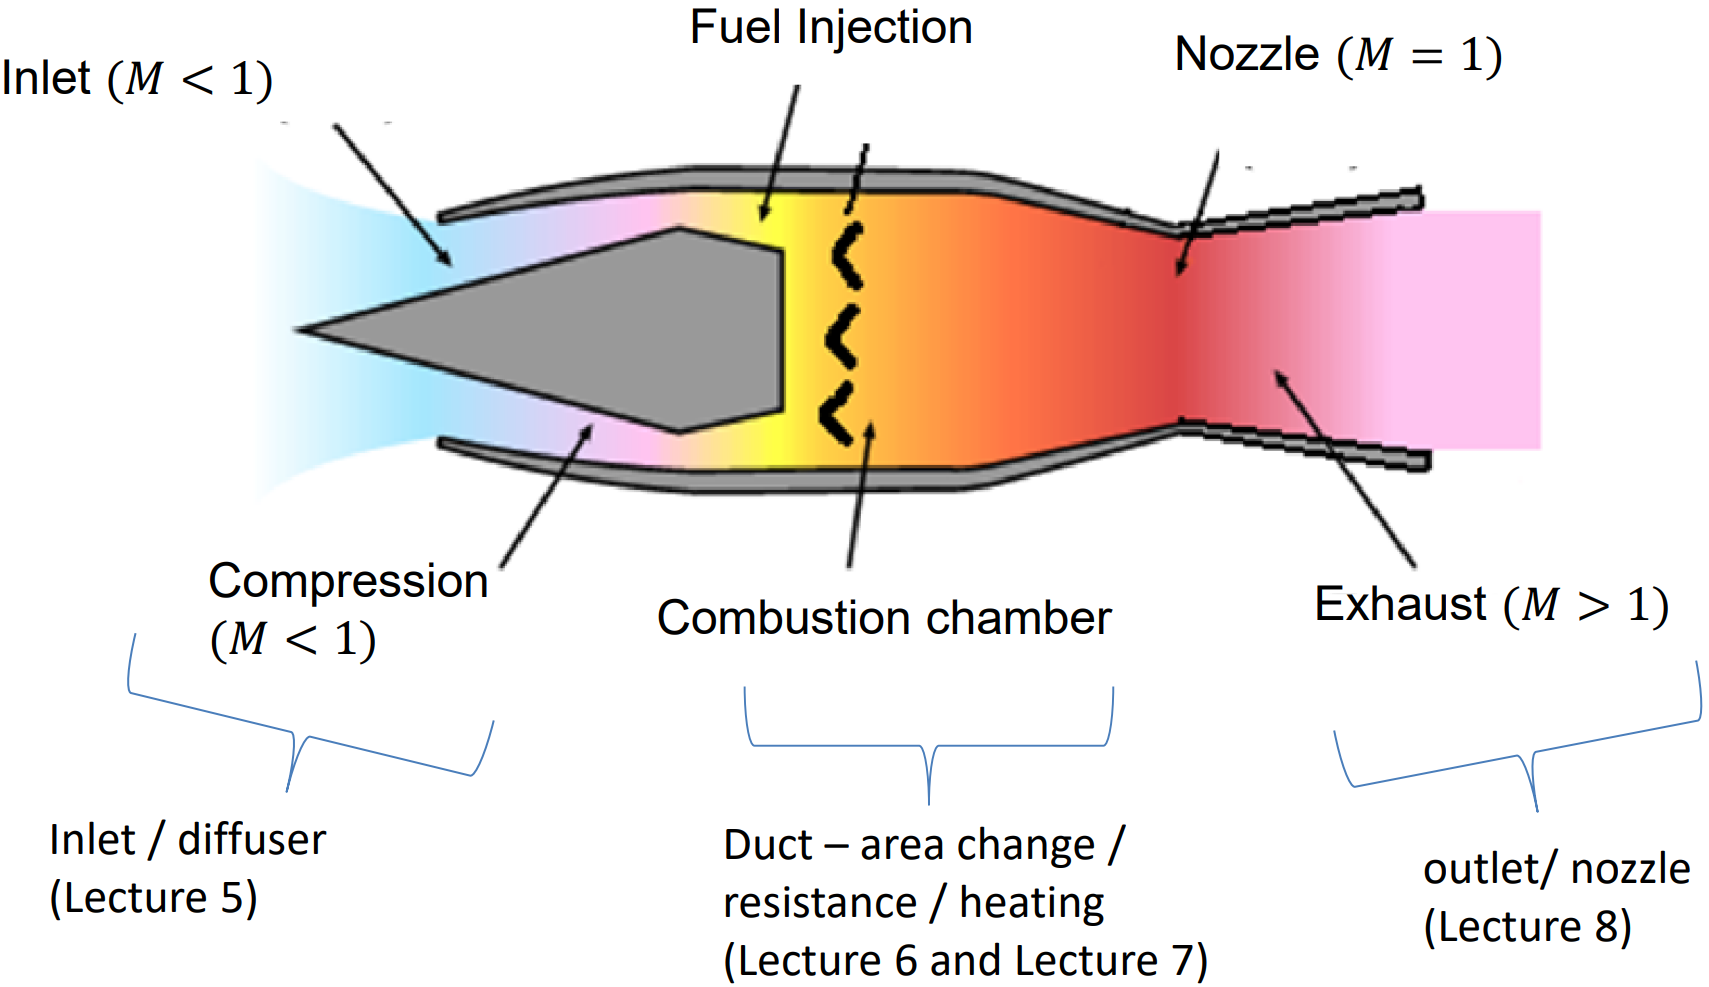
\includegraphics[width = \textwidth]{./img/diagram37.png}
    \caption{Components of a jet engine.}
\end{figure}
\subsection{Thrust from a jet/turbine}
\begin{figure}[H]
    \centering
    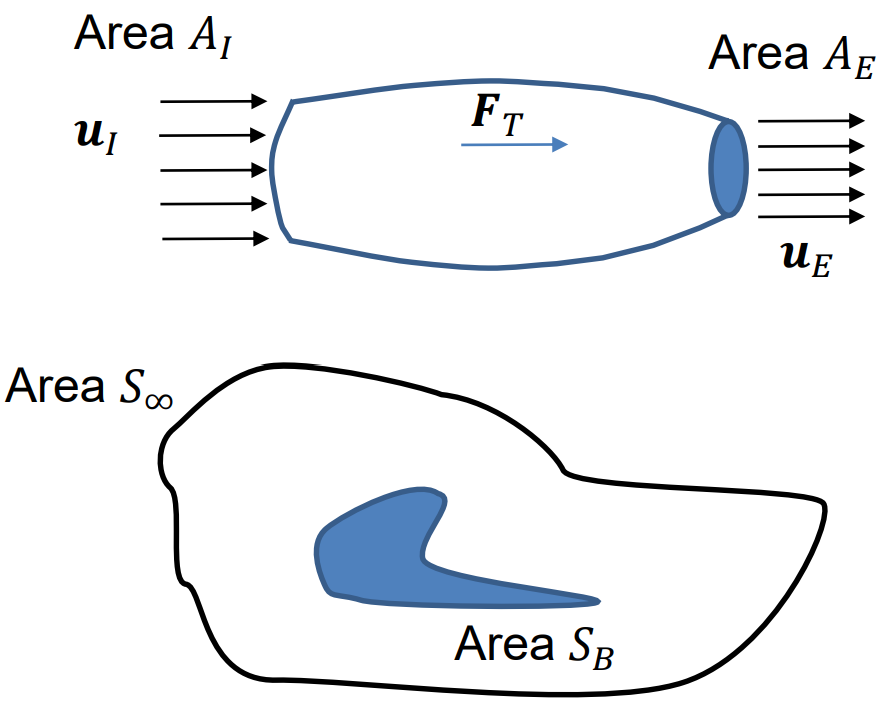
\includegraphics[width = 0.5\textwidth]{./img/diagram38.png}
    \caption{Inlet areas.}
\end{figure}
The thrust force on a body is determined by the integrated (pressure) force over its surface $S_B$:
\begin{gather}
    \underline{F}_T = \int_{S_{B}}\left(p\underline{\hat{n}}\right)\dif S
\end{gather}
From the conservation of momentum, the force can be expressed in terms of integrals over $S_{\infty}$ and $S_B$:
\begin{gather}
    \underline{F}_T = - \int_{S_{\infty}}\left(p \underline{\hat{n}}\right)\dif S + \int_{S_B + S_{\infty}}\left(\rho\left(\underline{u}\cdot\underline{\hat{n}}\right)\underline{u}\right)\dif S
\end{gather}
Taking a control surface that envelopes the body:
\begin{gather}
    \underline{F}_T \cdot \underline{\hat{x}} = A_Ep_E - A_1 p_1 + \dot{m} \left(u_E - u_1\right)
\end{gather}
\subsection{Purpose of an inlet}
\begin{figure}[H]
    \centering
    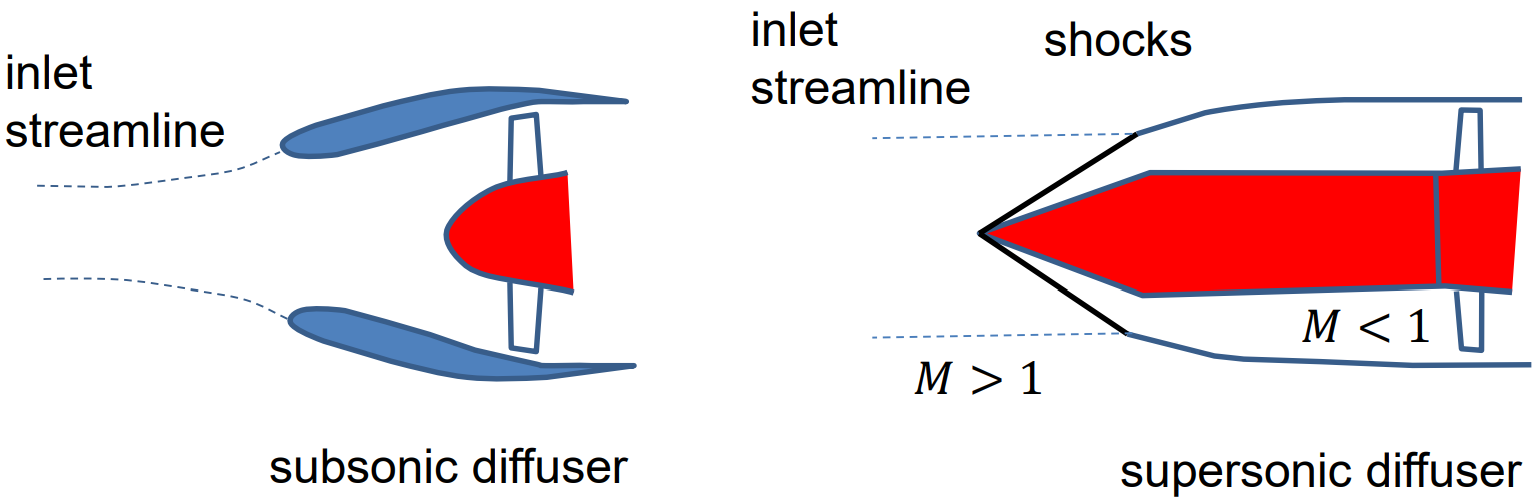
\includegraphics[width = 0.5\textwidth]{./img/diagram39.png}
    \caption{Inlet streamlines with various diffusers.}
\end{figure}
There are two requirements:
\begin{enumerate}
    \item Efficiency of engine depends on reducing losses (such as loss of stagnation pressure)
    \item Provide the required inlet mass flow (there are constraints to this). This is limited by choking of the inlet.
\end{enumerate}
\subsection{What do they look like?}
\begin{figure}[H]
    \centering
    \begin{minipage}{.5\textwidth}
        \centering
        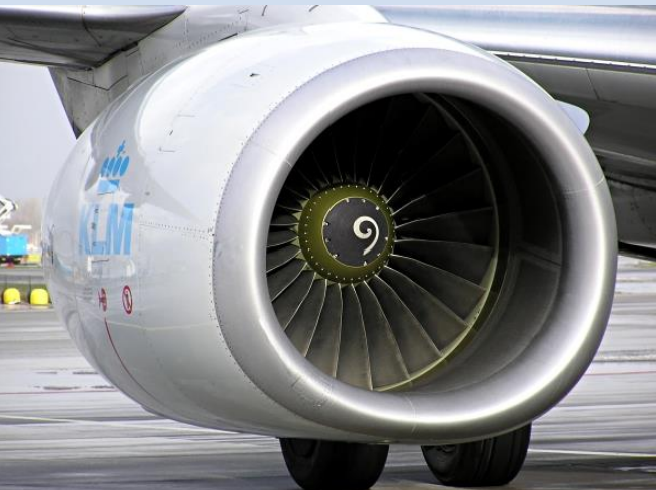
\includegraphics[width=.8\linewidth]{./img/diagram40.png}
        \captionof{figure}{Subsonic inlet.}
    \end{minipage}%
    \begin{minipage}{.5\textwidth}
        \centering
        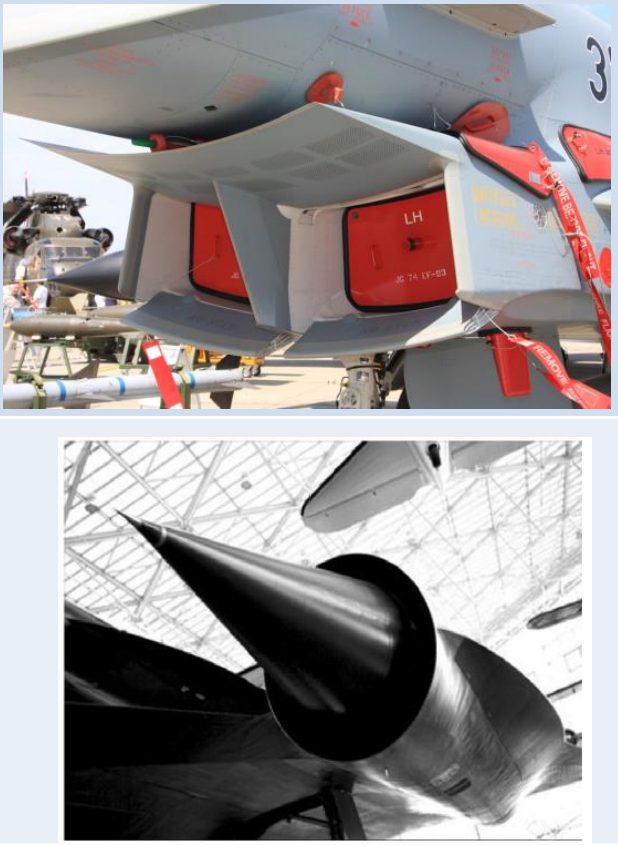
\includegraphics[width=.8\linewidth]{./img/diagram41.png}
        \captionof{figure}{Supersonic inlets.}
    \end{minipage}
\end{figure}
Modern jets are turbofans. This consists of a low speed fan and an inner high speed compressor. This is preferred because of the lower exhaust speed that is more efficient and gives rise to less noise.
\begin{figure}[H]
    \centering
    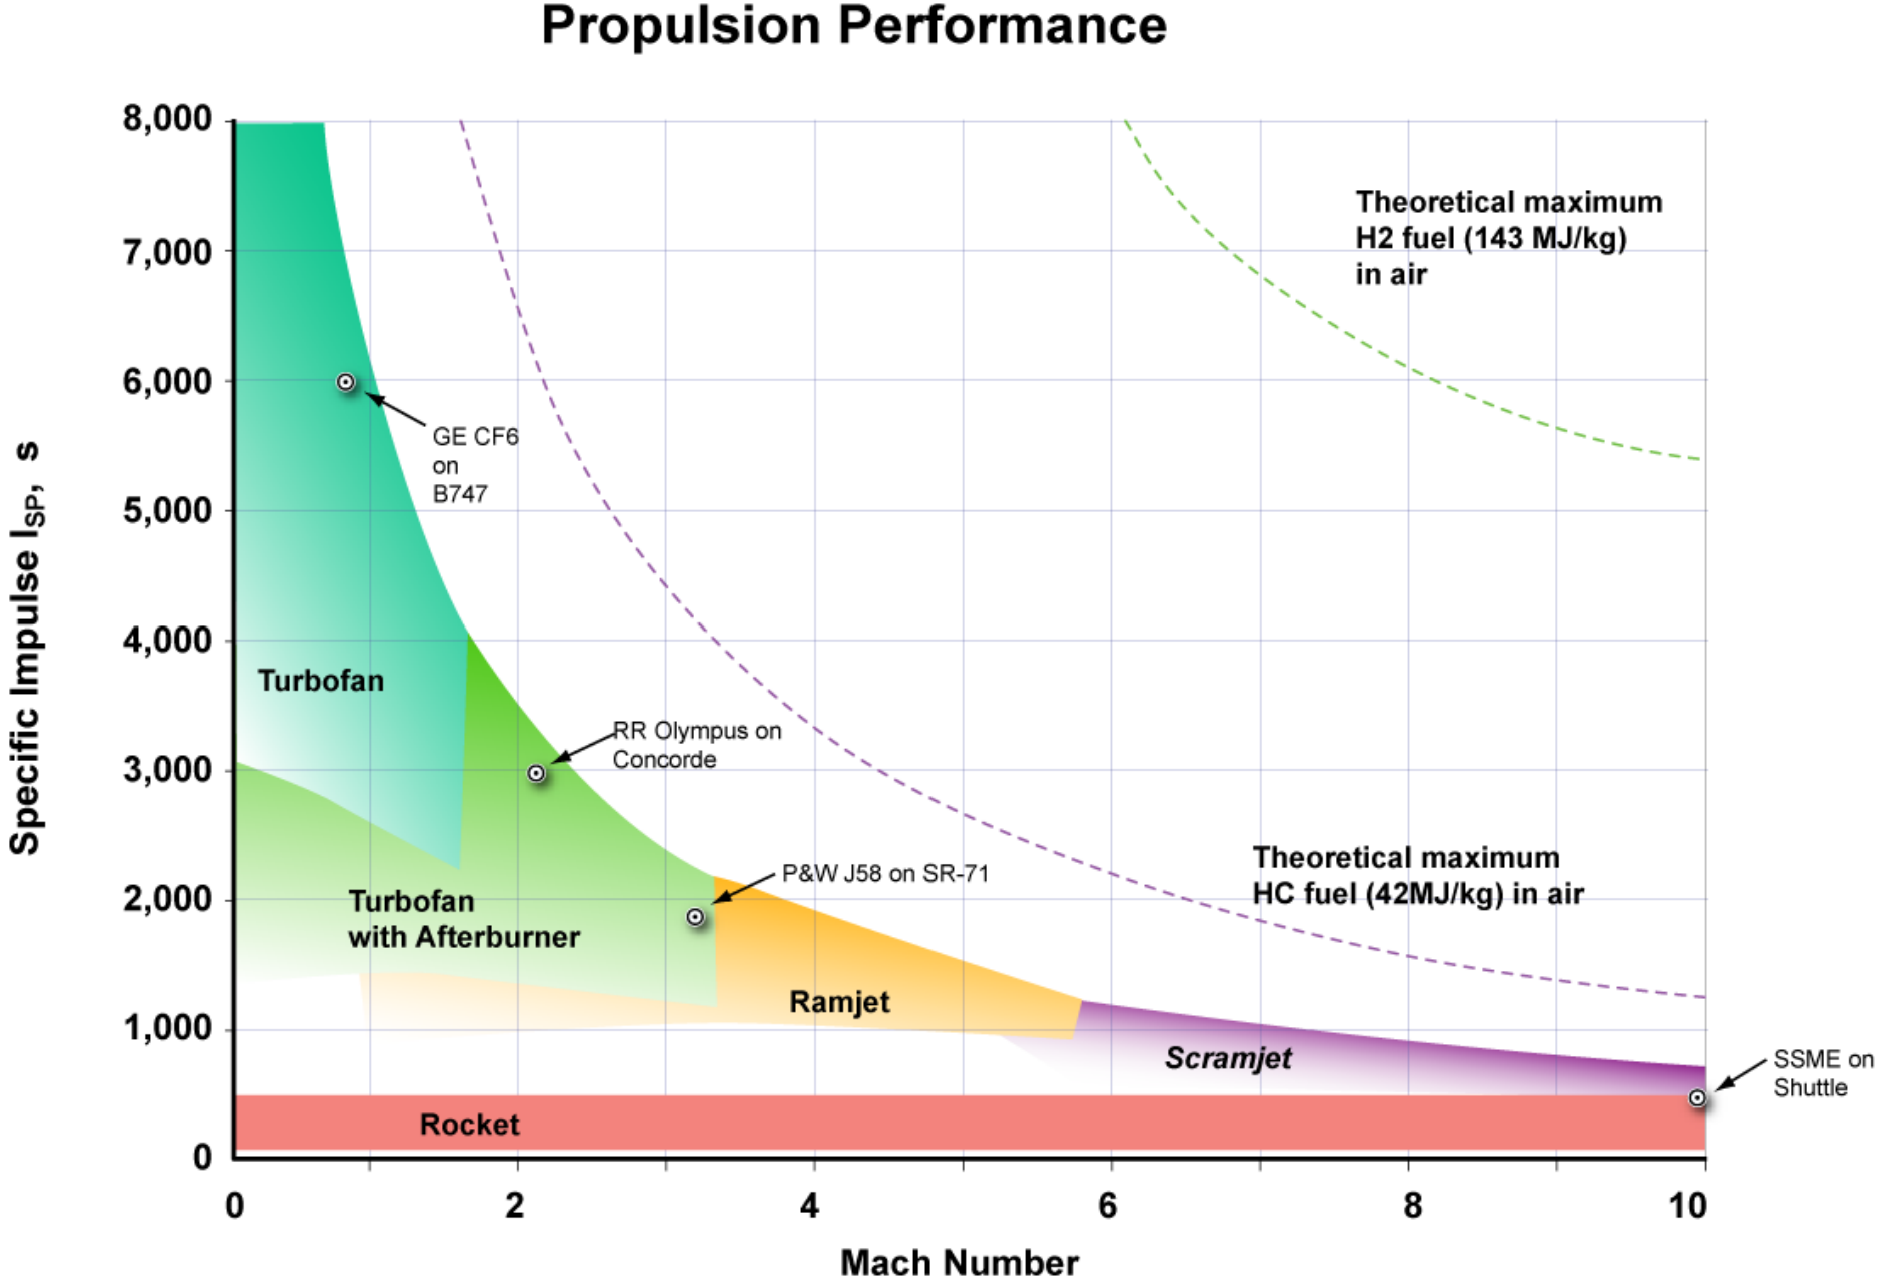
\includegraphics[width = 0.8\textwidth]{./img/diagram42.png}
    \caption{Graph to show propulsion performance for different inlet types.}
\end{figure}
Thrust divided by rate at which mass of propellant is consumed $\dfrac{F_T}{\dot{m}}$.
\section{Jet engines}
\begin{figure}[H]
    \centering
    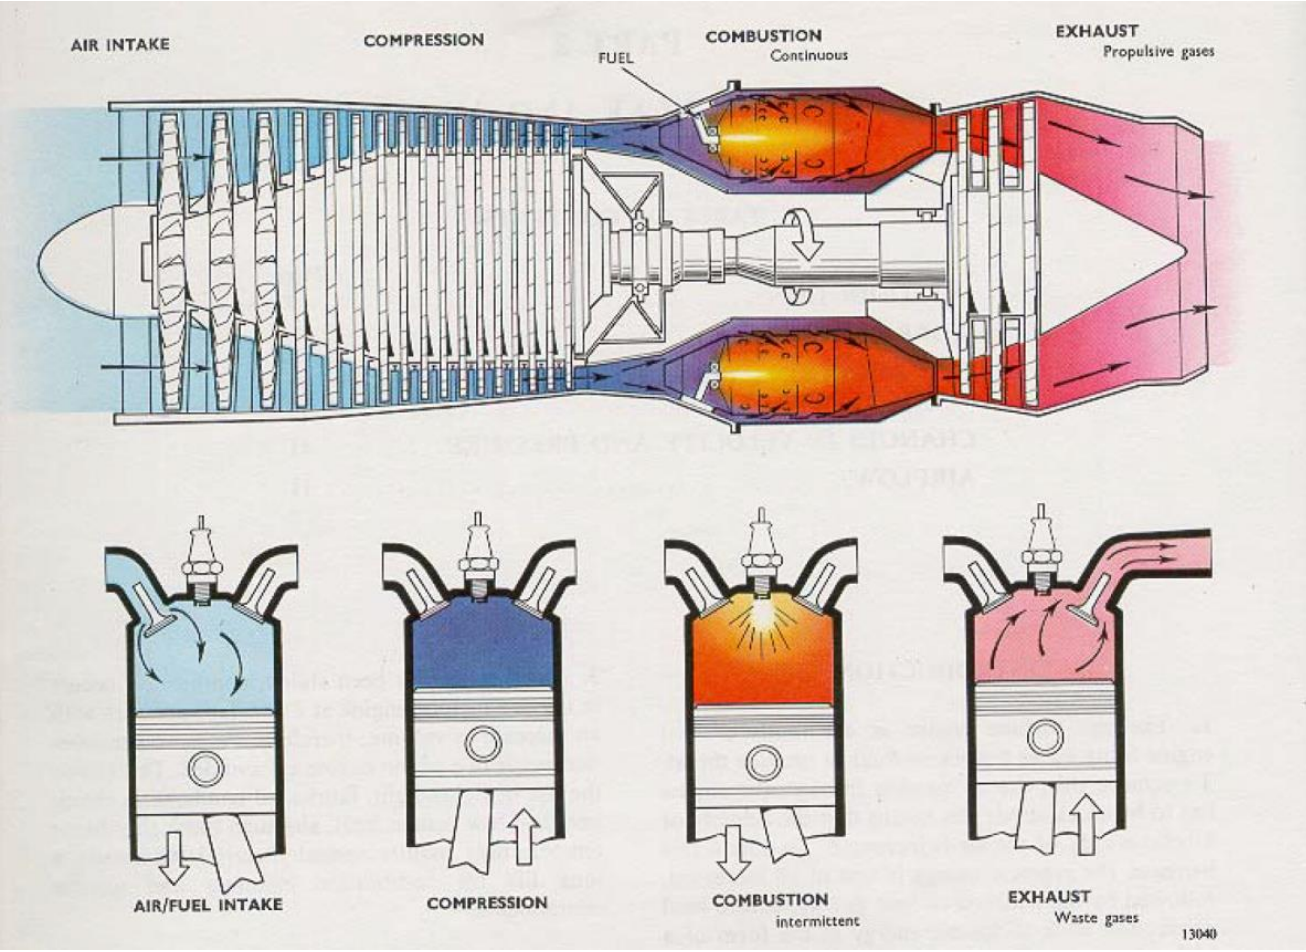
\includegraphics[width = 0.7\textwidth]{./img/diagram43.png}
    \caption{Jet engine.}
\end{figure}
In the first half - need high pressure, in the second half - need high velocity. There are four main components to a jet engine:
\begin{enumerate}
    \item Inlet
    \item Compression
    \item Combustion
    \item Exhaust
\end{enumerate}
Thrust:
\begin{enumerate}
    \item Exhaust gas
    \item Pushing the flow
\end{enumerate}
\subsection{Ramjet}
\begin{figure}[H]
    \centering
    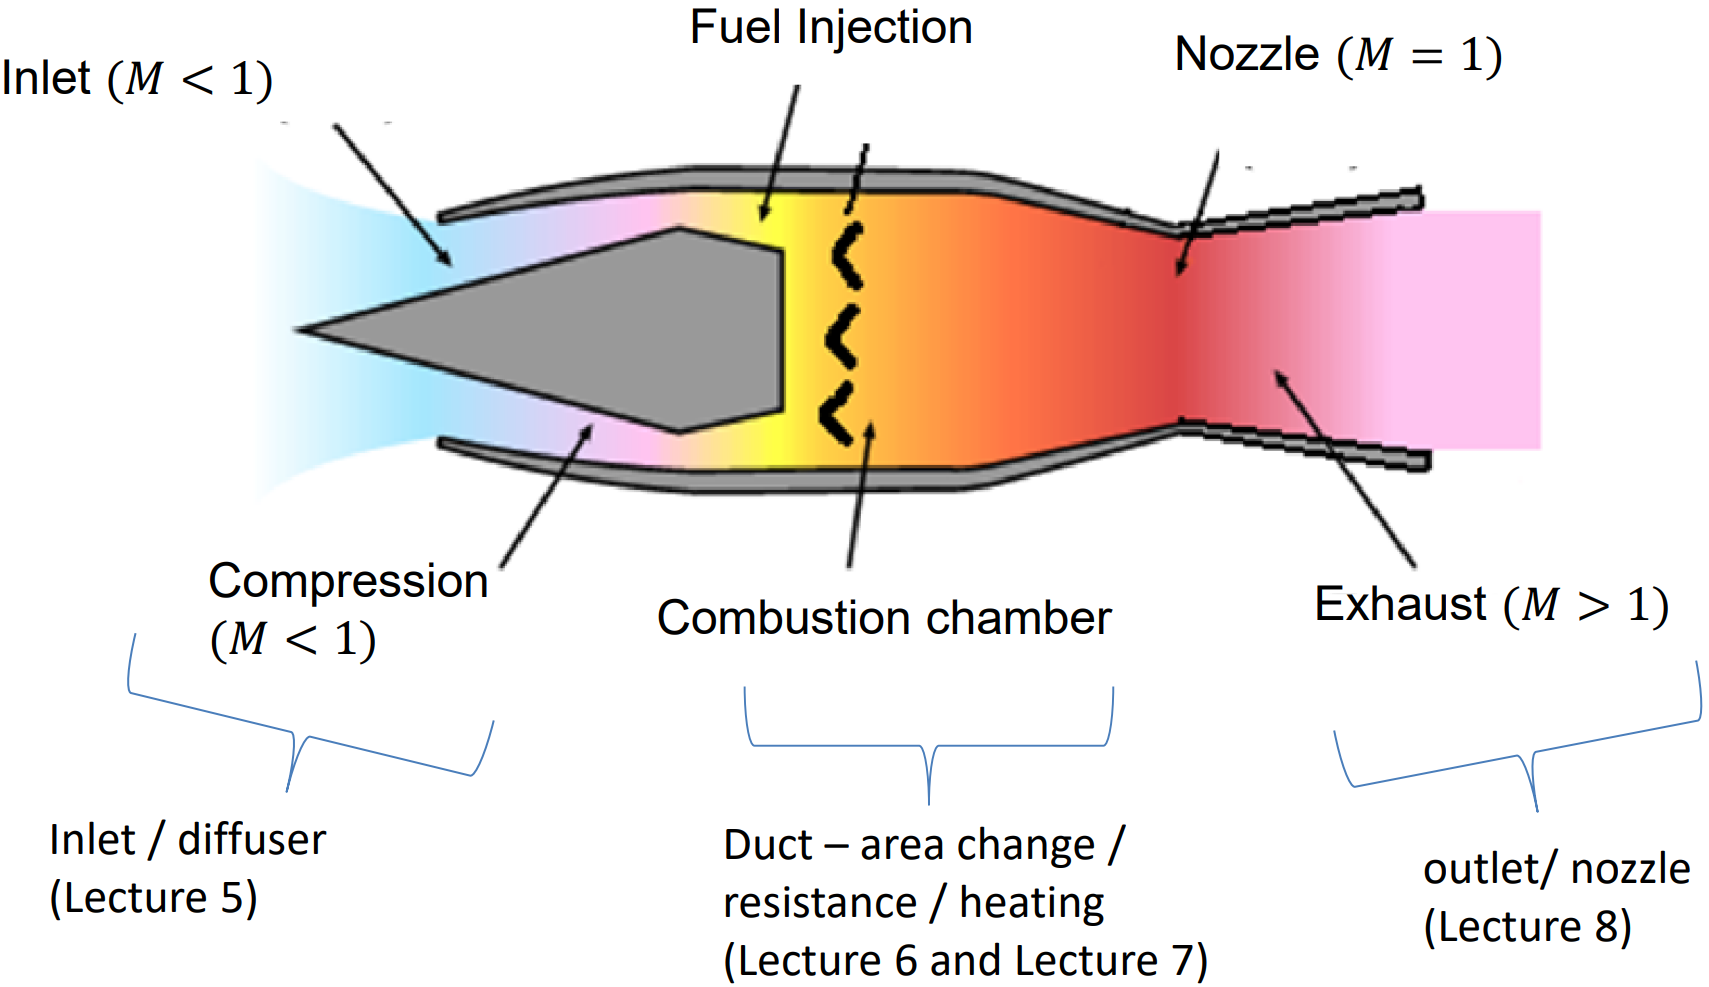
\includegraphics[width = 0.7\textwidth]{./img/diagram37.png}
    \caption{Ramjet.}
\end{figure}
This is a form of airbreathing jet engine that uses the engine's forward motion to compress incoming air without an axial compressor. Ramjets work most efficiently at supersonic speeds, around Mach 3 and can operate up to speeds of Mach 6 (\SI{7350}{\kilo\meter\per\hour}).
\subsection{Scramjet}
\begin{figure}[H]
    \centering
    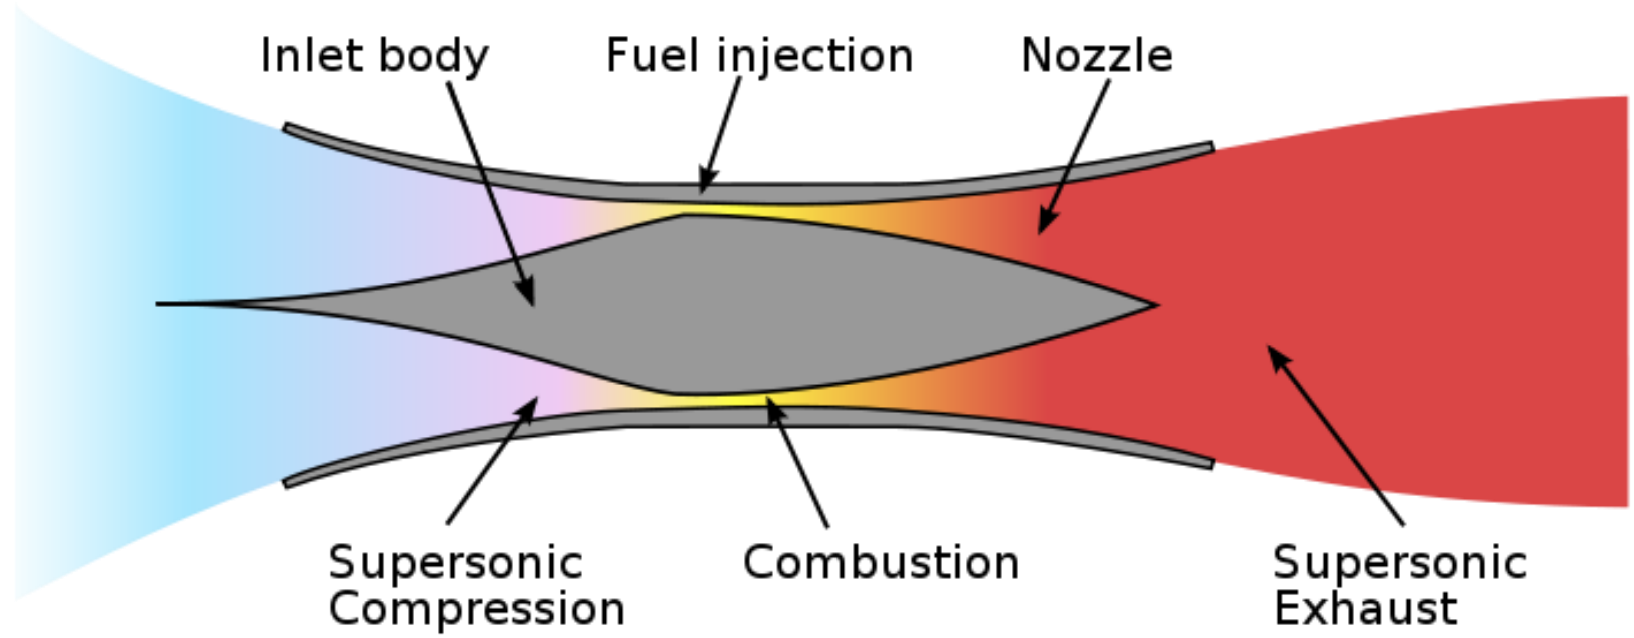
\includegraphics[width = 0.7\textwidth]{./img/diagram44.png}
    \caption{Scramjet.}
\end{figure}
This consists of a converging inlet, where incoming air is compressed; a combustor, where gaseous fuel is burned with atmospheric oxygen to produce heat. There is a diverging nozzle, where the heated air is accelerated to produce thrust. The flow is supersonic through the entire flow. The thrust is:
\begin{equation}
    F = \dot{m}\left(V_2 - V_1\right)
\end{equation}
Increasing pressure of airflow increases the potential energy. Increasing velocity increases kinetic energy. The purpose of the inlet, compressor and exhaust is to convert potential energy to kinetic energy.
\section{Inlet types}
\subsection{Subsonic}
\begin{figure}[H]
    \centering
    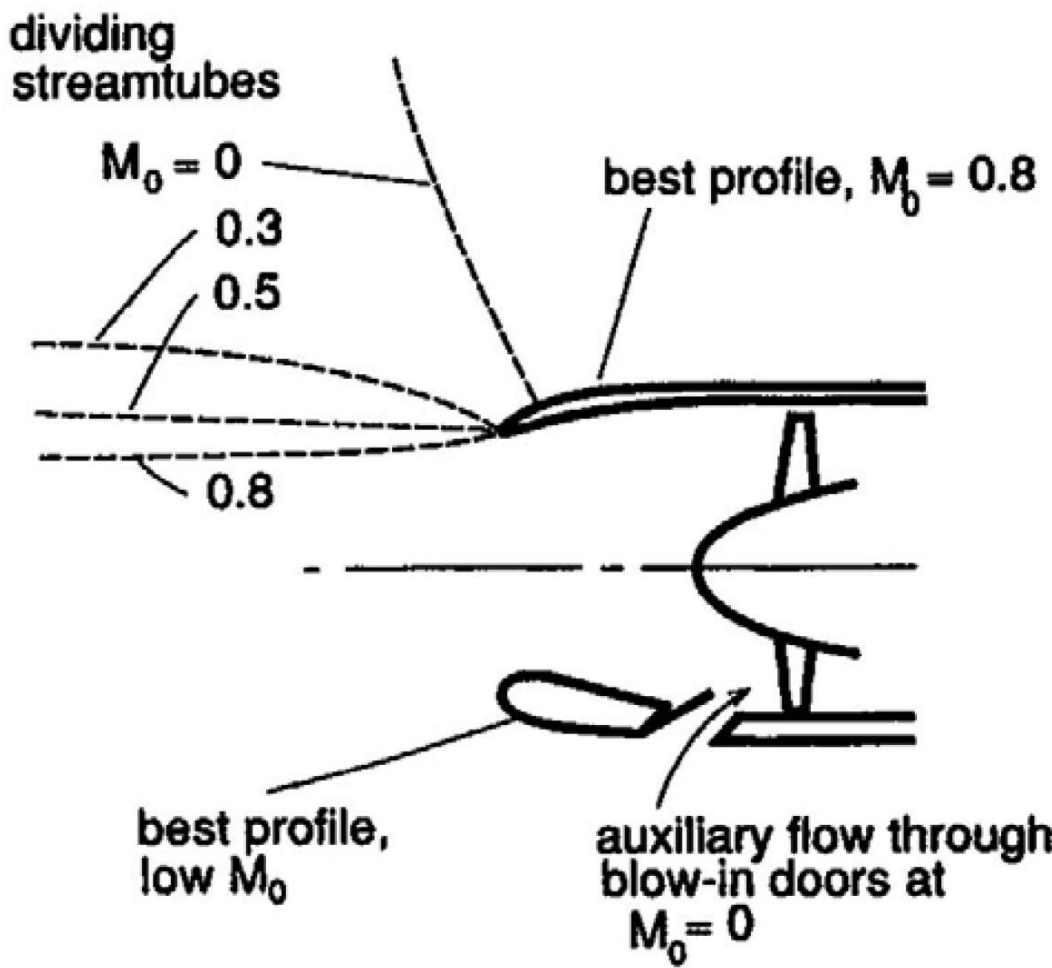
\includegraphics[width = 0.7\textwidth]{./img/diagram45.png}
    \caption{Subsonic inlet profile.}
\end{figure}
\subsection{Supersonic inlets}
An inlet for a supersonic aircraft, on the other hand, has a relatively sharp lip. The inlet lip is sharpened to minimise the performance losses from shock waves that occur during supersonic flight. For a supersonic aircraft, the inlet must slow the flow down to \textbf{subsonic} speeds before the air reaches the compressor.
\section{Simple normal shock inflow}
\begin{figure}[H]
    \centering
    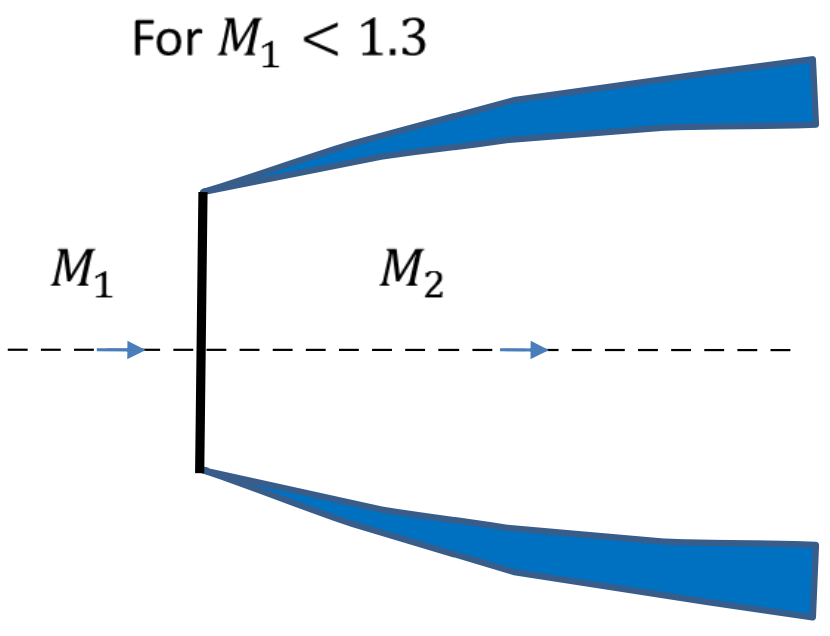
\includegraphics[width = 0.5\textwidth]{./img/diagram46.png}
    \caption{Simple normal shock inflow.}
\end{figure}
Relationship between flow properties upstream and downstream of shock:
\begin{gather}
    M^2_2 = \dfrac{1 + \frac{1}{2}\left(\gamma - 1\right)M^2_1}{\gamma M^2_1 - \frac{1}{2}\left(\gamma - 1\right)}\\
    \dfrac{p_2}{p_1} = 1 + \dfrac{2\gamma}{\gamma + 1}\left(M^2_1 - 1\right)
\end{gather}
\begin{figure}[H]
    \centering
    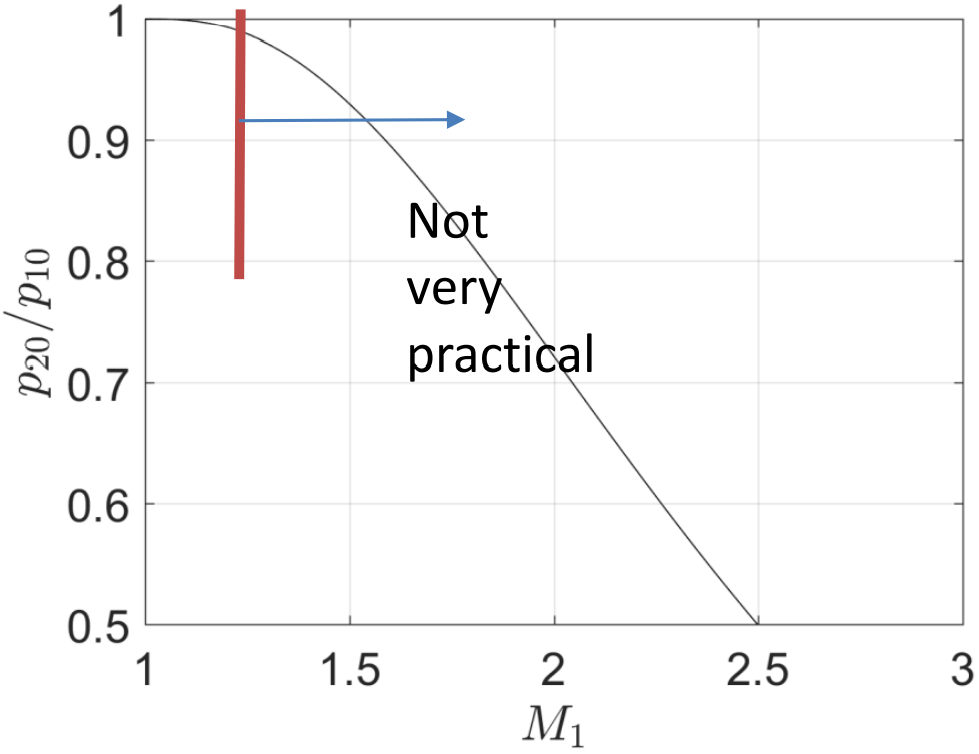
\includegraphics[width = 0.5\textwidth]{./img/diagram47.png}
    \caption{Graph to show ratio of stagnation pressure vs Mach number.}
\end{figure}
Ratio of stagnation pressure downstream to upstream of normal shock:
\begin{gather}
    \dfrac{p_{10}}{p_{20}} = \left(\dfrac{2\gamma M^2_1}{\gamma + 1}- \dfrac{\gamma - 1}{\gamma +1}\right)^{\frac{1}{\gamma - 1}}\left(\dfrac{\left(\gamma -1 \right)M^2_1+2}{\left(\gamma +1\right)M^2_1}\right)^{\frac{\gamma}{\gamma - 1}}
\end{gather}
\section{Basic concept - reflection of shock at wall}
\begin{figure}[H]
    \centering
    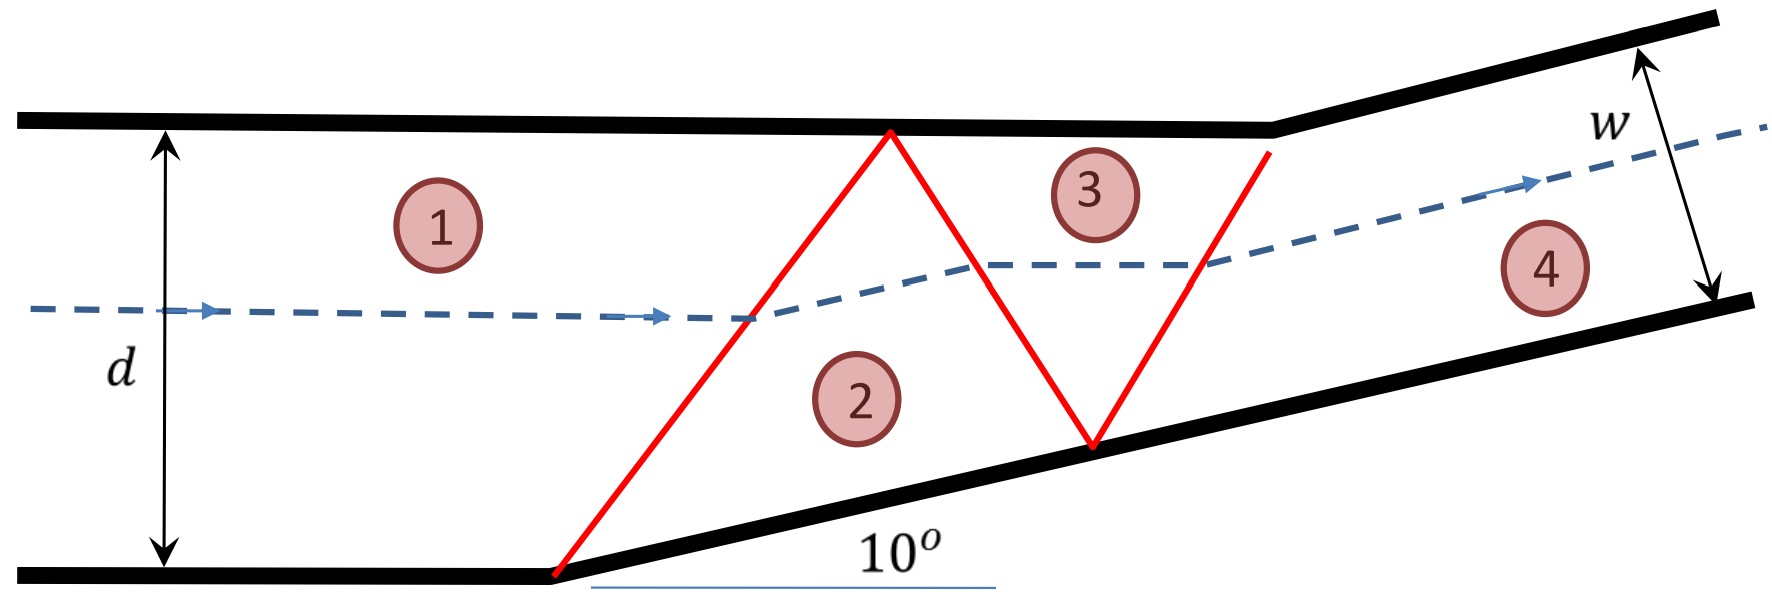
\includegraphics[width = 0.5\textwidth]{./img/diagram48.png}
    \caption{Diagram of shock at wall.}
\end{figure}
Example from Problem Sheet 2. The inlet Mach number is $M_1 = 2.8$. For a turning angle of \SI{10}{\degree}, calculate the width of the duct ($w$) in terms of the inlet width $d$, given that the shock cancels out at the corner.
\begin{table}[H]
    \centering
    \begin{tabular}{@{}llll@{}}
        \toprule
        Region 1    & Region 2                 & Region 3                  & Region 4                 \\ \midrule
        $M_1 = 2.8$ & $M_2 = 2.34$             & $M_3 = 1.94$              & $M_4 = 1.58$             \\
                    & $\zeta_2 = *$            & $\zeta_3 = *$             & $\zeta_4 = *$            \\
                    & $\dfrac{p_2}{p_1} = 2.0$ & $\dfrac{p_3}{p_2} = 1.82$ & $\dfrac{p_4}{p_3} = 1.*$ \\ \bottomrule
    \end{tabular}
    \caption{Mach numbers in different regions.}
\end{table}
\section{External vs internal compression}
\begin{figure}[H]
    \centering
    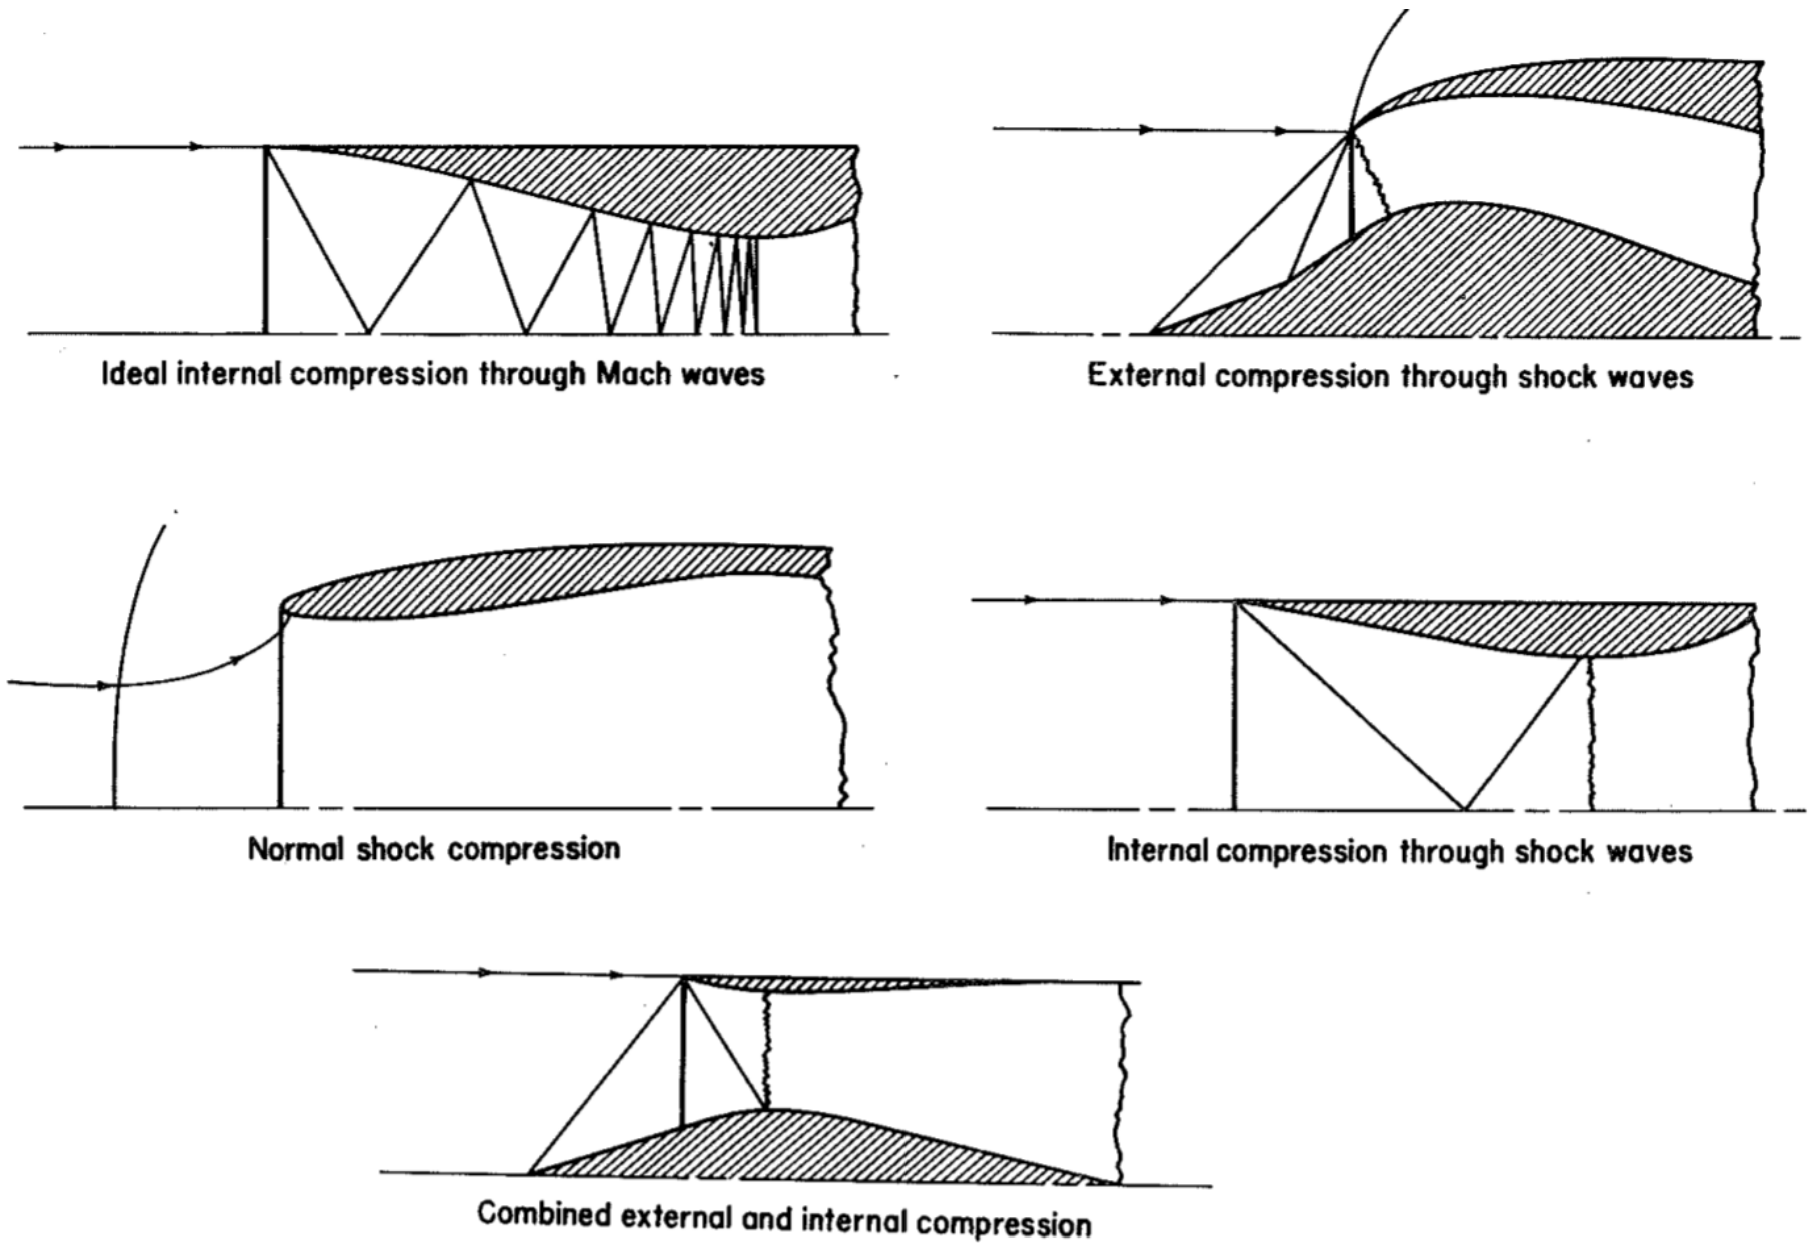
\includegraphics[width = \textwidth]{./img/diagram49.png}
    \caption{External vs internal compression.}
\end{figure}
\section{Strategy for increasing stagnation pressure}
\begin{figure}[H]
    \centering
    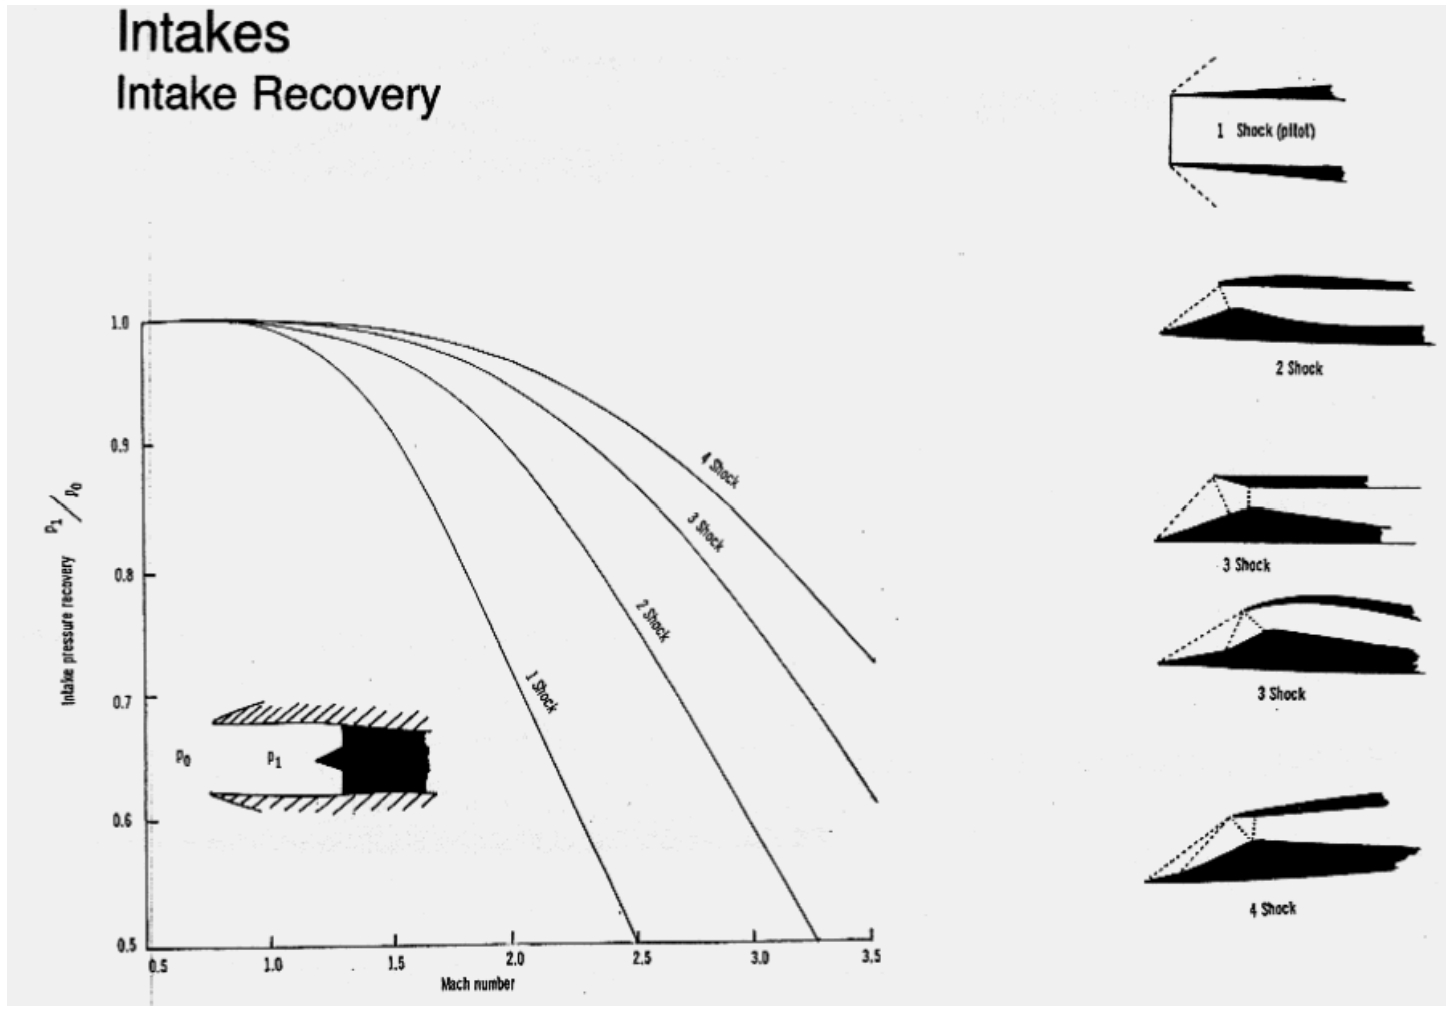
\includegraphics[width = 0.6\textwidth]{./img/diagram50.png}
    \caption{Intake recovery graph.}
\end{figure}
To increase the stagnation pressure after the compression stage, it is useful to compress the flow with a series of external and internal shocks. This shows the stagnation pressure ratio due to a series of shocks which are of equal strength. Equal strength means that:
\begin{gather}
    \dfrac{p_2}{p_1} = \dfrac{p_3}{p_2} = \dfrac{p_4}{p_3} = ...
\end{gather}
\subsection{Optimal choice}
The shocks are set up so that they tend to meet at the edge of the cowl. This is to:
\begin{enumerate}
    \item minimise spillage
    \item minimise buzz - oscillations in the inlet
    \item minimise loss of stagnation pressure
\end{enumerate}
We tend to ensure that the ratio of stagnation pressure across the shocks is the same (i.e. they have the same strength).
\section{Oblique diffusers}
\begin{figure}[H]
    \centering
    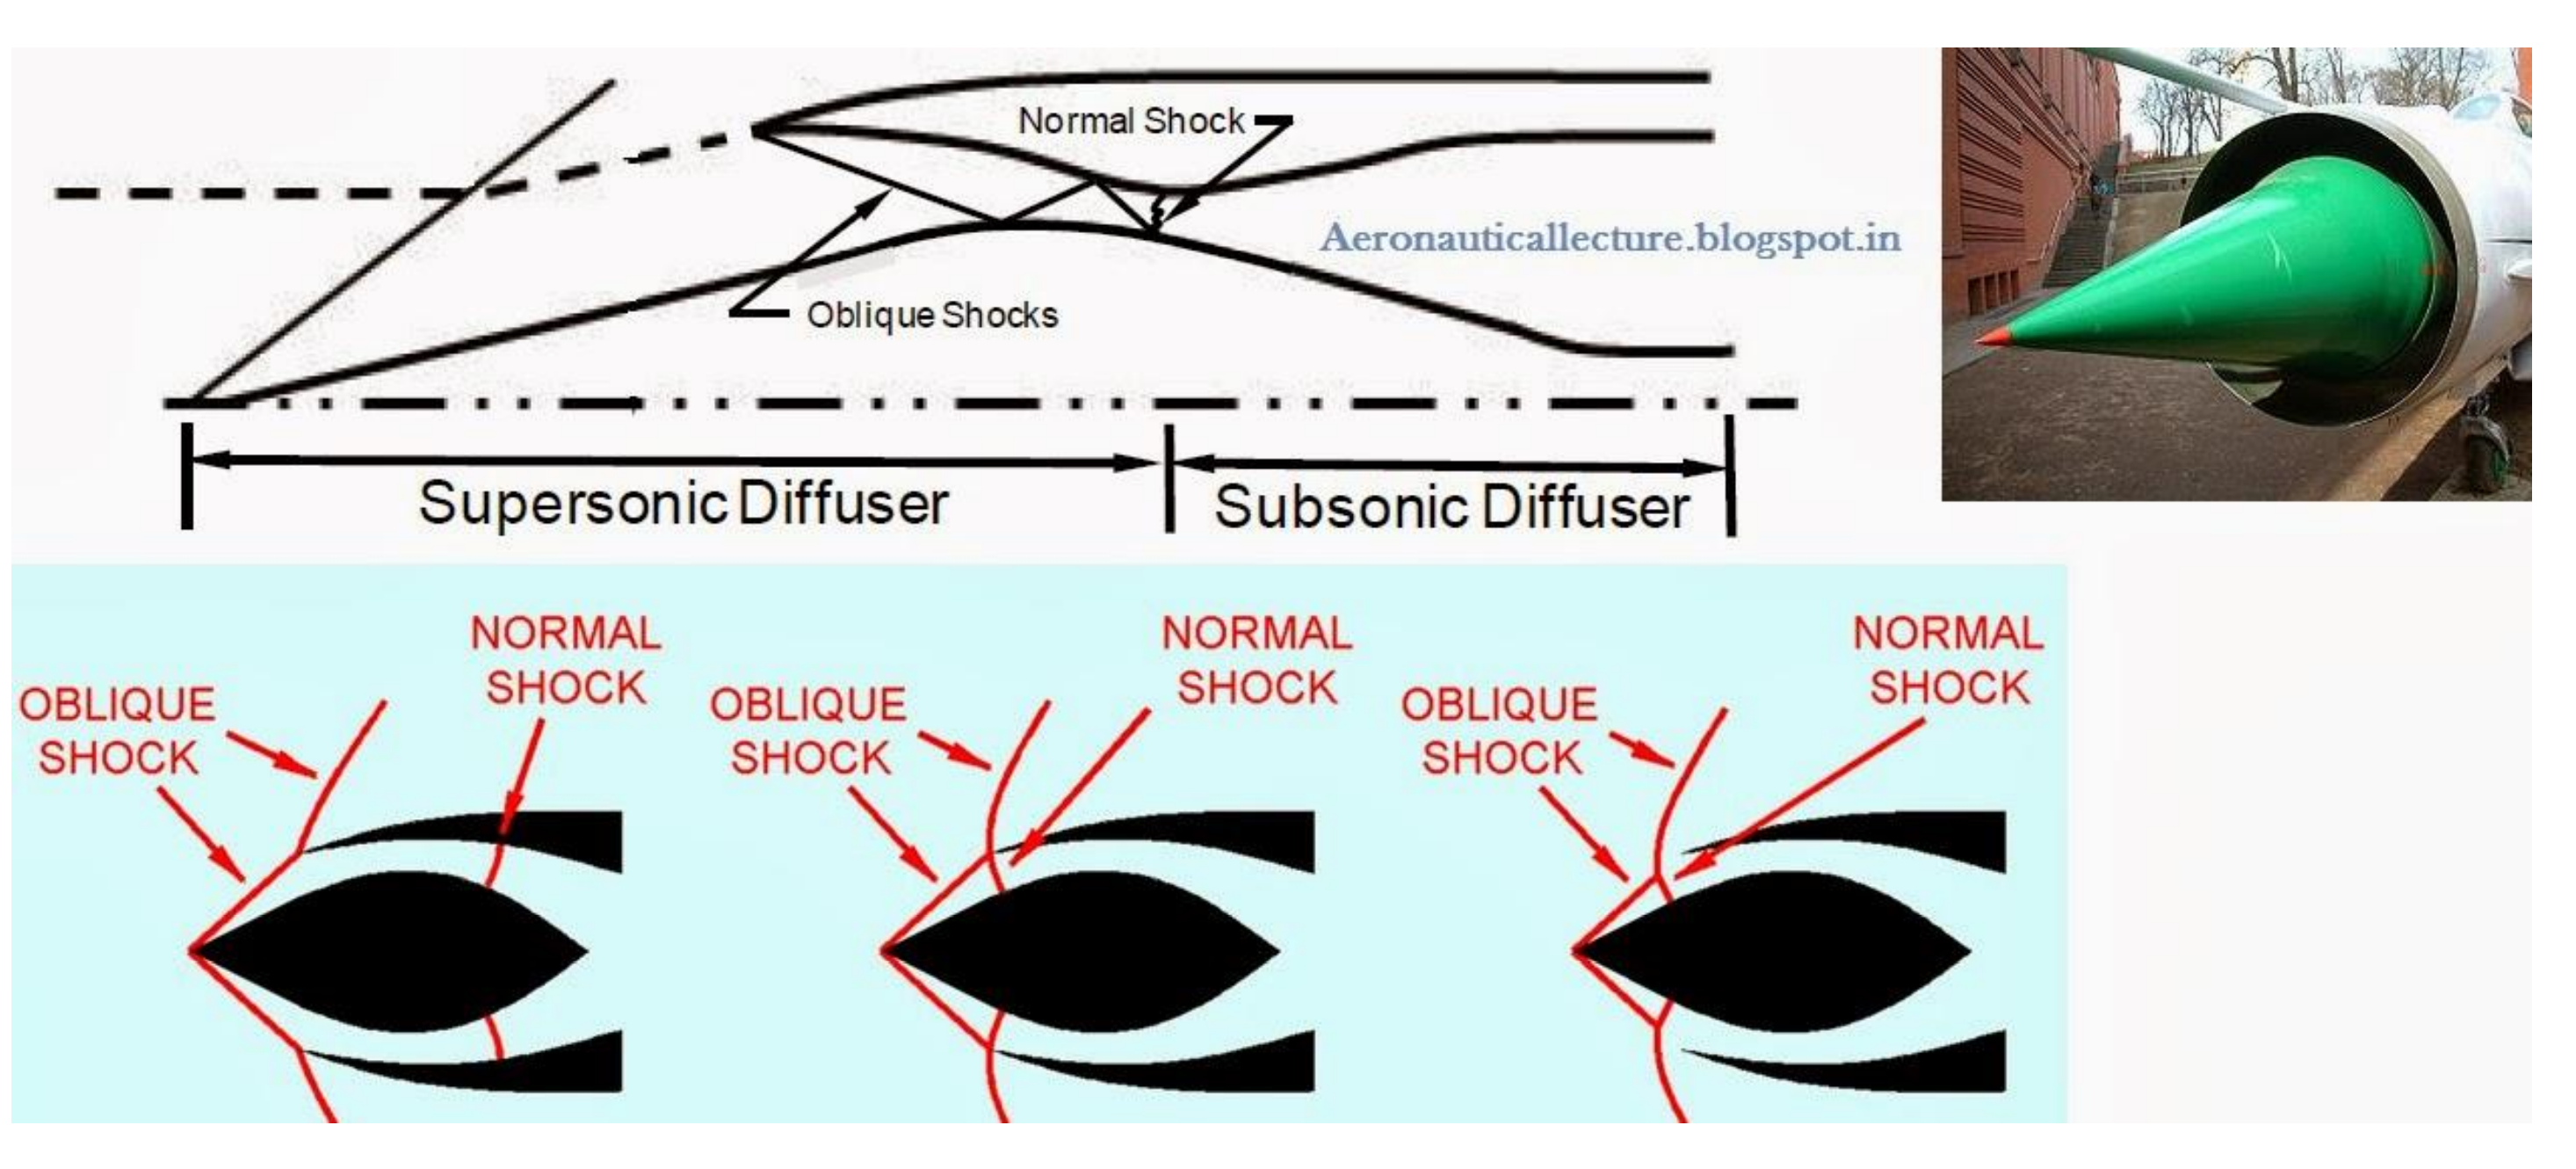
\includegraphics[width = \textwidth]{./img/diagram51.png}
    \caption{Oblique diffusers.}
\end{figure}
\subsection{Adaptation}
A movable cone called a 'spike' is used. For subsonic flow, the spike is pushed forward. When the aircraft accelerated past Mach 1.6, an internal jackscrew moved the spike up \SI{66}{\centi\meter} inwards, directed by an analog air inlet computer that took into account pitot-static system, pitch, roll, yaw and angle of attack. Moving the spike tip drew the shock wave riding on it closer to the inlet cowling until it touched just slightly inside the cowling.